% %%%% Benefit of reasoning about 
% \subsection{Motivation of Reasoning about Adaptivity}
% % 
In Section~\ref{subsec:intro-motivation},
I firstly introduce the motivation of reasoning about the \emph{adaptivity} quantity property 
for adaptive data analysis program.
% analyzing 
In order to analyze this \emph{adaptivity} property for the adaptive data analysis, there are 3 challenges
% problems encountered.
introduced next in Section~\ref{subsec:intro-adapt}.
% I introduce these three problems
% and the full-spectrum analysis methodologies developed according to these problems 
Targeting to the three challenges, I introduce my full-spectrum analysis methodologies accordingly.
Concretely, the full-spectrum analysis is developed through the language formalization,
the execution-based analysis, and the static-based program analysis.
%
Based on the implementation and experimental results on my full-spectrum analysis, 
I propose three significant 
further features can be improved 
% in the analysis methodologies 
in Section~\ref{subsec:intro-improve}, 
and plan to finish these improvements 
before the final defense.
%
 % Next, based on the implementation and experimental results, I proposed two significant 
 % further features can be improved for my analysis framework, and plan to finish the improvement 
 % before the final defense.
 %
 Then, in Section~\ref{subsec:intro-cost}, through two observations, I introduce the motivations and methodologies
 for the accurate full-spectrum program resource cost analysis.
%   with implicit cost decreases.
% \\
% 1. traditional program's resource cost analysis failed to consider the case where the program's cost could decrease 
% implicitly, 
% \\
% 2. and 
% % when there isn't a dependency relation between variables.
% the resource consumption during the program 
% execution increases and particularly decreases implicitly in the same way as the program's adaptivity, 
% % Specifically, in line 5 
% % where the list is re-written and the heap consumption is decreased implicitly. 
% % This implicit decrease 
% % of the cost works the same as the program's adaptivity decreases.
% I'm interested in improving the accuracy of the program's general resource cost analysis
% by 
% % onto the program's resource cost analysis. 
% % Use this framework,
% Through the generalized \emph{adaptivity} analysis framework.
% I will give
% a more accurate resource cost estimation by taking the program's implicit resource cost into consideration, comparing 
% to the worst case cost analysis in a traditional way.
 For this work, the analysis framework design and the implementation is expected to be done before the final thesis.
%  Finally, the 
 Section~\ref*{subsec:intro-cfl} introduces the 
%  the interest in showing that
CFL-Reachability problem and the motivations of 
%  CFL-Reachability problems can be solved by reducing them to my adaptivity analysis framework. 
solving it by reducing into my full-spectrum adaptivity analysis framework. 
 This work is planned to start before the final defense and develop further after.
 % based on the study on the traditional way of performing data flow and control analysis,
 % I identify the similarity between the traditional way of performing data flow and control analysis, and the 
 % adaptivity analysis. 
 % Specifically I identify the similarity between 
 % solving the feasible path problem in the analysis by reducing CFL-reachability problems,
 % and the way of computing the adaptivity in my static analysis framework.
 % Motivated by this observation, 
 % % I'm Interested
 % % the, There are similarities between
 % % solving the data flow problem by reducing to CFL-reachability problem,
 % % resource analysis through reducing to CFL-reachability problem, 
 % I'm interested in showing that
 % CFL-reachability problems can be solved by reducing them to my adaptivity analysis framework. 
 % This work is planned to start before the final defense and develop further sophisticated after.

\subsection{Adaptive Data Analysis}
\label{subsec:intro-motivation}


Consider a dataset $X$ consisting of $n$ independent samples from some unknown population $\dist$. How can I ensure that the conclusions are drawn from $X$ \emph{generalize} to the population $\dist$? Despite decades of research in statistics and machine learning on methods for ensuring generalization, there is an increased recognition that many scientific findings generalize poorly (e.g. 
\cite{Ioannidis05,GelmanL13}
). While there are many reasons a conclusion might fail to generalize, one that is receiving increasing attention is \emph{adaptivity}, which occurs when the choice of method for analyzing the dataset depends on previous interactions with the same dataset~\cite{GelmanL13}.

 Adaptivity can arise from many common practices, such as exploratory data analysis, using the same data set for feature selection and regression, and the re-use of datasets across research projects. Unfortunately, adaptivity invalidates traditional methods for ensuring generalization and statistical validity, which assume that the method is selected independently of the data. The misinterpretation of adaptively selected results has even been blamed for a ``statistical crisis'' in empirical science~\cite{GelmanL13}.
% ~\cite{GelmanL13}.

A line of work initiated by \cite{DworkFHPRR15}, \cite{HardtU14} posed the question: Can I design \emph{general-purpose} methods that ensure generalization in the presence of adaptivity, together with guarantees on their accuracy? 
The idea that has emerged in these works is to use randomization to help ensure generalization. 
Specifically, these works have proposed to mediate the access of an adaptive data analysis to the data utilizing queries from some pre-determined family (I will consider here a specific family of queries often called "statistical" or "linear" queries) that are sent to a 
\emph{mechanism} which uses some randomized process to guarantee that the result of the query does not depend too much on the specific
sampled dataset. 
%
\begin{figure}
 \centering
 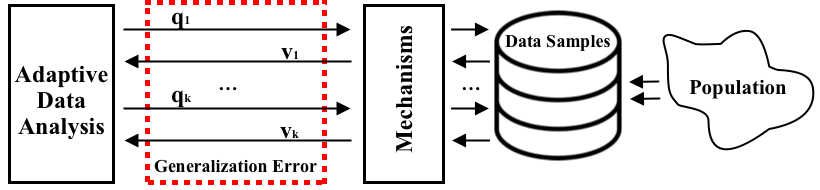
\includegraphics[width=0.7\columnwidth]{figures/data_analysis_model.png}
 \caption{Overview of our Adaptive Data Analysis model.}
 \label{fig:adaptivity-model-overview}
\vspace{-0.5cm}
\end{figure}
This guarantees that the result of the queries generalizes well. 
This approach is described in Figure~\ref{fig:adaptivity-model-overview}, where
I have a population that I'm interested in studying, and a dataset containing individual samples from this population. The adaptive data analysis I'm interested in running has access to the dataset through queries of some pre-determined family (e.g., statistical or linear queries) mediated by a mechanism. 
This mechanism uses randomization to reduce the generalization error of the queries issued to the data.
This line of work has identified many new algorithmic techniques for ensuring generalization in adaptive data analysis, leading to algorithms with greater statistical power than all previous approaches. 
Common methods proposed by these works include the addition of noise to the result of a query, data splitting, etc. 
Moreover, these works have also identified problematic strategies for adaptive analysis, showing limitations on the statistical power one can hope to achieve. 
Subsequent works have then further extended the methods and techniques in this approach and further extended the theoretical underpinning of this approach, 
e.g.~\cite{dwork2015reusable,dwork2015generalization,BassilyNSSSU16,UllmanSNSS18,FeldmanS17,jung2019new,SteinkeZ20,RogersRSSTW20}.
%

A key development in this line of work is that the best method for ensuring generalization in an adaptive data analysis depends to a large extent on the number of \emph{rounds of adaptivity}, the depth of the chain of queries. 
As an informal example, the program $x \leftarrow \query_1(D);y \leftarrow \query_2(D,x);z \leftarrow \query_3(D,y)$ has three rounds of adaptivity, since $\query_2$ depends on $D$ not only directly because it is one of its input but also via the result of $\query_1$, 
which is also run on $D$, and similarly, $\query_3$ depends on $D$ directly but also via the result of $\query_2$, which in turn depends on the result of $\query_1$. 
The works I discussed above showed that not only does the analysis of the generalization error depend on the number of rounds, 
but knowing the number of rounds allows one to choose methods that lead to the smallest possible generalization error. 

% \mg{Check the following - also the plots need to be on the same scale!}
For example, these works showed that when an adaptive data analysis uses a large number of rounds of adaptivity then a low generalization error can be achieved by the mechanism of 
adding to the result of each query Gaussian noise scaled to the number of rounds. When instead an adaptive data analysis uses a small number of rounds of adaptivity then a low generalization error can be achieved by using more specialized methods, such as the data splitting mechanism or the reusable holdout technique from~\cite{DworkFHPRR15}.
To better understand this idea, I show in Figure~\ref{fig:generalization_errors} two experiments showcasing these situations. 
More precisely, in Figure~\ref{fig:generalization_errors}(a) shows the results of a real-world analysis
with two rounds of adaptivity. 
This analysis can be seen as a classifier that first runs 500 non-adaptive queries on the first 500 attributes of the data, looking for correlations between the attributes and a label, and then runs one last query which depends on all these correlations. 
Without any mechanism, the generalization error is pretty large, and the lower generalization error is achieved when the data-splitting method is used. 
In Figure~\ref{fig:generalization_errors}(b) shows the results of a specific analysis
with four hundred rounds of adaptivity. 
This analysis can be seen as a classifier that at each step runs an adaptive query based on the result of the previous ones. 
Again, without any mechanism, the generalization error is pretty large, and the lower generalization error is achieved when the Gaussian noise is used. 
{\small
\begin{figure}
\centering
\begin{subfigure}{.48\textwidth}
\begin{centering}
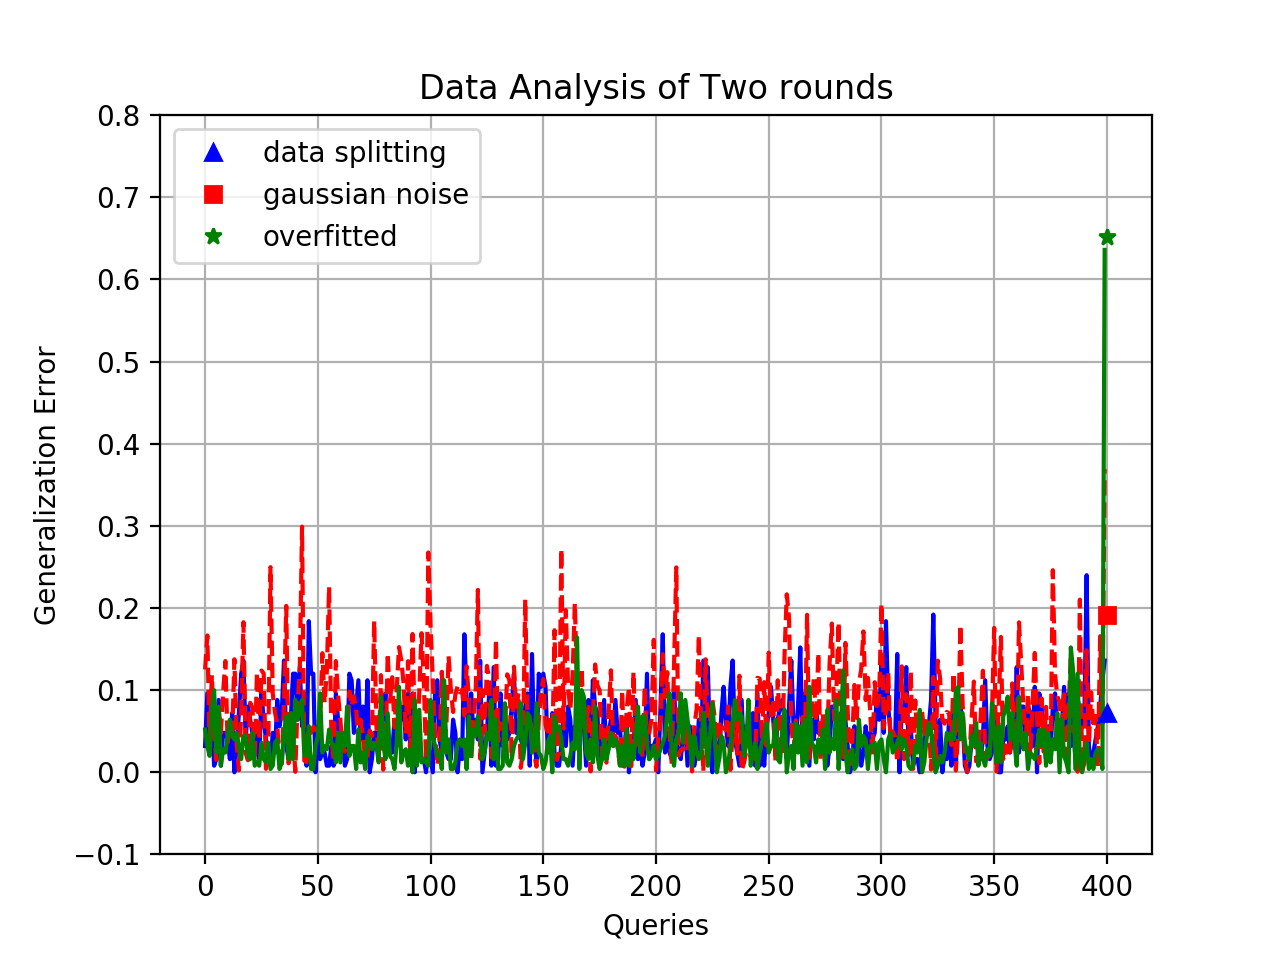
\includegraphics[width=0.9\textwidth]{figures/tworound.png}
\caption{}
\end{centering}
\end{subfigure}
%}
\quad
\begin{subfigure}{.48\textwidth}
\begin{centering}
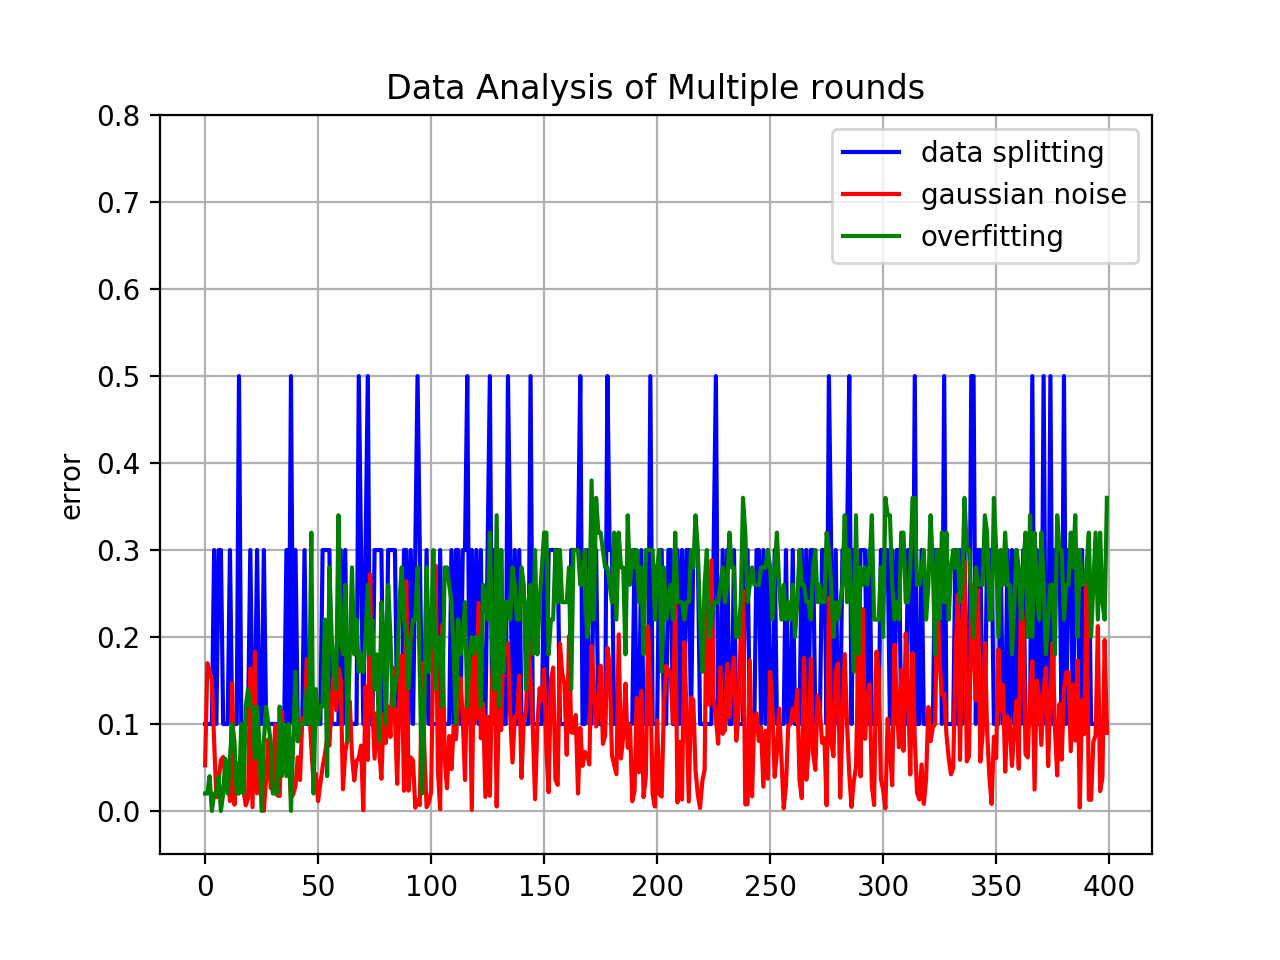
\includegraphics[width=0.9\textwidth]{figures/multipleround.png}
\caption{}
\end{centering}
\end{subfigure}
\vspace{-0.4cm}
 \caption{
 The generalization errors of two adaptive data analysis examples, under different choices of mechanisms.
 (a) Data analysis with adaptivity 2, 
 (b) Data analysis with adaptivity 400. 
}
\label{fig:generalization_errors}
\vspace{-0.5cm}
\end{figure}
}
%gap
This scenario motivates us to explore the design of program analysis techniques that can be used to estimate the number of \emph{rounds of adaptivity} that a program implementing a data analysis can perform. These techniques could be used to help a data analyst in the choice of the mechanism to use,
and they
could ultimately be integrated into a tool for adaptive data analysis such as the \emph{Guess and Check} framework by~\cite{RogersRSSTW20}. 
%
In order to analyze this property, there is mainly three property. 
In this proposal, I will first focus on analyzing 
this adaptivity property for the program is based on solving the three problems specifically as follows.

\subsection{Full-Spectrum Adaptivity Analysis and Methodology}
\label{subsec:intro-adapt}
There are mainly three challenges in order to analyze this adaptivity property, 
and the full-spectrum analysis of this property is 
% In this proposal, I will first focus on analyzing 
% this adaptivity property for the program based on solving 
developed w.r.t. the three challenges accordingly.

\begin{enumerate}
 \item
 \textbf{Adaptive Data Analysis Formalization}
The first challenge is \emph{how to define formally} a model for adaptive data analysis which is general enough to support the methods I discussed above and would permit to formulate the notion of adaptivity these methods use. 
I take the approach of designing a programming framework for submitting queries to some \emph{mechanism} giving access to the data mediated by one of the techniques I mentioned before, e.g., adding Gaussian noise, randomly selecting a subset of the data, using the reusable holdout technique, etc. 
In this approach, a program models an \emph{analyst} asking a sequence of queries to the mechanism. The mechanism runs the queries on the data applying one of the methods discussed above and returns the result to the program. The program can then use this result to decide which query to run next. 
% Overall, I'm interested in controlling the generalization of the results of the queries which are returned by the mechanism, by means of adaptivity. 

\textbf{Methodology}
Motivated by this, I present a while-like language named {\tt Query While} language with extensions on query requests in Section~\ref{sec:language}.

\item 
\textbf{Adaptivity Formalization}
The second challenge is \emph{how to define the adaptivity of a given program}.
Intuitively, a query $Q$ may depend on another query $P$, if there are two values that $P$ can return which affect in different ways the execution of $Q$. 
For example, as shown in \cite{dwork2015reusable}, and as I did in our example in Figure~\ref{fig:generalization_errors}(a), one can design a machine learning algorithm for constructing a classifier that first computes each feature's correlations with the label via a sequence of queries, and then constructs the classifier based on the correlation values. 
If one feature's correlation changes, the classifier depending on features is also affected. 
This notion of dependency builds on the execution trace as a \emph{causal history}. 
In particular, I'm interested in the history or provenance of a query up until this is executed, I'm not then concerned about how the result is used --- except for tracking whether the result of the query may further cause some other query. 
This is because I focus on the generalization error of queries and not their post-processing. % 

\textbf{Methodology}
To formalize this intuitive \emph{adaptivity} as a quantitative program property, 
I develop an execution-based analysis in Section~\ref{sec:dynamic}.
% I first consider all the possible evaluations of a program --- I do this by 
% I use a trace semantics recording the execution history of programs on some given input --- and I create a dependency graph, where the dependency between different variables (query is also assigned to a variable) is explicit and track which variable is associated with a query request. 
% I then enrich this graph with weights describing the maximal number of times each variable is evaluated in a program evaluation starting with an initial state. The adaptivity is then defined as the length of the walk visiting most query-related variables on this graph. 
% Through two aspects: the execution-based analysis and static-based program analysis.
% In the execution-based analysis, I will formalize the intuitive notion of \emph{adaptivity} as a quantitative 
% property of programs. This analysis is developed 
 This execution-based analysis is designed in three steps through different methodologies as follows,
 \begin{enumerate}
 \item The first step is to analyze the \emph{dependency relation} between every query, 
 through the methodology of semantic data dependency analysis.
 %
 Specifically through a trace semantics recording the execution history of programs on given input,
 % --- and I create a dependency graph, 
 the dependency between different variables (query is also assigned to a variable) is explicitly tracked and 
 analyzed.
%   and 
%   which variable is associated with a query request. 
% I then enrich this graph with weights describing the maximal number of times each variable is evaluated in a program evaluation starting with an initial state. The adaptivity is then defined as the length of the walk visiting most query-related variables on this graph. 
% In the execution-based analysis, I will formalize the intuitive notion of \emph{adaptivity} as a quantitative 
% property of programs. This analysis is developed 
% \\
 \item The second step is to analyze the \emph{dependency quantity} 
%  analysis, 
based on the \emph{dependency relation} above.
This analysis is developed through the methodology of execution-based reachability bound analysis.
% \\
 \item The last step is the intuitive \emph{adaptivity} quantity analysis, 
 according to the two analysis results above, specifically \emph{dependency relation} and \emph{dependency quantity}.
 This step 
%  is developed through 
gives the formal \emph{adaptivity} definition as the analysis result. \\
 Specifically, this analysis is developed through creating a dependency graph firstly. 
 In this graph, the dependency between different variables (query is also assigned to a variable) 
 is explicit and track which variable is associated with a query request. 
 This dependency comes from the \emph{dependency relation} from the first step analysis.
 \\
Then, I enrich this graph with 
weights describing the maximal number of times each variable is evaluated in a program evaluation starting with an initial state. 
This weight comes from the \emph{dependency quantity} from the second step analysis results.
\\
 The adaptivity is then defined as the length of the walk visiting most query-related variables on this graph. 
 \end{enumerate}
\item 
\textbf{Adaptivity Estimation}
The third challenge is \emph{how to estimate the adaptivity of a given program}. 
The adaptive data analysis model I consider and our definition of adaptivity suggest that for this task I can use a program analysis that is based on some form of dependency analysis. This analysis needs to take into consideration:
1) the fact that, in general, a query $Q$ is not a monolithic block but rather it may depend, through the use of variables and values, on other parts of the program. 
Hence, it needs to consider some form of data flow analysis. 
2) the fact that, in general, the decision on whether to run a query or not may depend on some other value. Hence, 
 it needs to consider some form of control flow analysis.
3) the fact that. in general, I'm not only interested in whether there is a dependency or not, but in the length of the chain of dependencies. 
Hence, it needs to consider some quantitative information about the program dependencies. % {A quick example is that: I store the result of query $Q_1$ in variable $x$ and use variable $y$ to record the result of query $Q_2$. I want to construct the third query $Q_3$ which relies on the value stored in $x$, let us say, $Q_3$ will ask for the sum of the first column of a table if $x$ is positive and the sum of the second column otherwise. In this situation, I need data flow analysis. On the other hand, if I need the value of $y$ to help us decide whether I should ask $Q_3$, for example, I ask the third query if $y$ is odd, and do not ask if $y$ is even. Naturally, to be able to handle this case, control flow analysis comes into play. Formally speaking, }

\textbf{Methodology}
To address these considerations and be able to estimate a sound upper bound on the adaptivity of a program, 
I will develop a static program analysis in Section~\ref{sec:static}, named {\THESYSTEM}.
This analysis combines data flow and control flow analysis with reachability bound analysis.
% ~\cite{GulwaniZ10}. 
This new program analysis gives tighter bounds on the adaptivity of a program than the ones one would achieve 
by directly using the data and control flow analyses or the ones that one would achieve 
by directly using reachability bound analysis techniques alone. 
% Specifically as follows in the same 
It is developed in 3 aspects similar to the execution-based analysis 
while through static program analysis techniques.
A sound estimated result is given in each part, which is summarized as follows.
\begin{enumerate}
\item The data dependency relation analysis through the static data flow analysis technique.
\item The dependency quantity analysis through the static program reachability bound analysis techniques.
\item 
% The program  estimation, 
The static analysis for adaptivity, specifically estimating the \emph{adaptivity} formalized in the execution-based analysis.
%  is presented in Section~\ref{subsubsec:static-reachability}.
% the program adaptivity estimation, 
In this analysis, I construct a program-based dependence graph for approximating the execution-based graph
%  in Section~\ref{subsubsec:dynamic-adapt}.
Then, based on this graph, I design an algorithm
%  based on the results estimated above, 
computing the adaptivity upper bound soundly 
and accurately.
\end{enumerate}
%%%%% To reason about%
\end{enumerate}% \\

\subsection{Further Works}
\subsubsection{Towards Full-Spectrum Adaptivity Analysis Extension}
\label{subsec:intro-improve}
Based on the implementation and experimental results of the basic full-spectrum analysis,
%  on the $\THESYSTEM$,
I plan to focus on the following three further features which can be extended and improved.
%  in my full-spectrum analysis.
\begin{enumerate}
    \item Extension of the {\tt Query While} Language with inter-procedure call.
    \item In the execution-based \emph{adaptivity},
    I plan to improve the precision of the intuitive \emph{adaptivity} formalization,
%  in the formal  model 
in the meantime extend this analysis with inter-procedure call.
\item In static \emph{adaptivity} analysis, I plan to give a tighter estimated upper bound on \emph{adaptivity}
%  give a tighter estimated upper bound 
Specifically, I will focus on improving the accuracy of the static \emph{dependency quantity} analysis in the second step through 
path sensitive reachability bound analysis techniques. 
% \item In the third step of static program analysis, I will improve the accuracy of the adaptivity computation algorithm,
% compute a tighter adaptivity upper bound as well.
\end{enumerate}
\subsubsection{Towards Accurate Full-Spectrum Program Resource Cost Analysis}
\label{subsec:intro-cost}
Moving towards the area of general program resource cost analysis,
% Then, motivated by the two following aspects, 
there are two interesting observations as follows.
% I'm interested 
These two observations motivated me in 
% improving the accuracy of the program's general resource cost analysis
improving the accuracy of the program's general resource cost analysis
by generalizing this \emph{adaptivity} analysis framework.
\begin{itemize}
 \item Firstly, in a traditional program's resource cost analysis,
 There are two categories of program cost analysis, type-system based and data-flow/control-flow analysis based. 
 In the type-system design-based works, they \cite{GustafssonEL05} and \cite{hoffmann_jost_2022}, explicit abstraction or data structure de-allocation in order to save or reduce the cost.
 
 Both of the
 works in these two areas fail to recognize the case where program resource consumption is decreased implicitly.
 \item The resource consumption during the program 
 execution increases and particularly decreases implicitly in the same way as the program's adaptivity. This is explained in detail through an example in Section~\ref*{sec:generalization}.
\end{itemize}
% F
% Then, through two observations,
% that 
% firstly, traditional program's resource cost analysis failed to consider the case where the program's cost could decrease 
% implicitly, and 
% % when there isn't a dependency relation between variables.
% the resource consumption during the program 
% execution increases and particularly decreases implicitly in the same way as the program's adaptivity, 
% % Specifically, in line 5 
% % where the list is re-written and the heap consumption is decreased implicitly. 
% % This implicit decrease 
% % of the cost works exactly the same as the program's adaptivity decrease.
% I'm interested in improving the accuracy of the program's general resource cost analysis
% by generalizing my \emph{adaptivity} analysis framework.
 % onto the program's resource cost analysis. 
 % Use this framework,
 Based on the observations above, 
 I plan to develop
 an accurate program general resource cost analysis framework through generalizing my full-spectrum \emph{adaptivity} analysis.
 This framework can give more accurate cost bound than traditional worst-case resource cost estimation methods,
 by taking the program's implicit resource cost into consideration.
%  compared 
%  to the worst-case cost analysis in the traditional way.

\subsubsection{Towards Solving the CFL-Reachability Problem}
\label{subsec:intro-cfl}
Still in the area of general program resource cost analysis,
the traditional methodology of performing data flow and control analysis and 
computing the program resource cost is
% Finally, based on the study on the traditional way of performing data flow and control analysis,
to reduce the analysis problem into the CFL-reachability problems.
% Finally, based on the study on the traditional way of performing data flow and control analysis,
According to this, 
I identify 
% the similarity between the traditional way of performing data flow and control analysis and the 
that there are some similarities between the traditional way of estimating the program resource cost and 
the adaptivity.
%  Specifically, I identify the similarity between 
%  solving the feasible path problem in the analysis by reducing 
Specifically, there are similarities between solving the CFL-reachability problems they reduced to,
%  CFL-reachability problems,
 and the way of computing the adaptivity in 
%  my static analysis framework.
the third step of $\THESYSTEM$.
 Motivated by this, 
 % I'm Interested
 % the, There are similarities between
 % solving the data flow problem by reducing to CFL-reachability problem,
 % resource analysis through reducing to CFL-reachability problem, 
 I'm interested in showing that
 CFL-reachability problems can be solved by reducing to my adaptivity analysis framework.
% I identify the similarity between the traditional way of performing data flow and control analysis and the 
%  adaptivity analysis. 
%  Specifically, I identify the similarity between 
%  solving the feasible path problem in the analysis by reducing CFL-reachability problems,
%  and the way of computing the adaptivity in my static analysis framework.
%  Motivated by this observation, 
%  % I'm interested
%  % the, There are similarities between
%  % solving the data flow problem by reducing to CFL-reachability problem,
%  % resource analysis through reducing to CFL-reachability problem, 
%  I'm interested in showing that
%  CFL-reachability problems can be solved by reducing them to my adaptivity analysis framework.


\subsection{Proposal Structure}
\label{subsec:intro-structure}

To sum up, this proposal covers the following topic in each following section.
\begin{enumerate}
\item A while-like language extended with query request feature, named {\tt Query While} Language, 
used to implement 
the adaptive data analysis in Section~\ref{sec:language}.
\item A formal adaptivity model through execution-based adaptivity analysis in Section~\ref{sec:dynamic}.
\item A static program analysis algorithm named {\THESYSTEM} in Section~\ref{sec:static}.
\item Three proposed further features to be improved in Section~\ref{sec:furthers}, 
based on the 
% formal adaptivity model and {\THESYSTEM}, 
 full-spectrum adaptivity analysis.
%  presented in Section~\ref{sec:language},~\ref{sec:dynamic} and~\ref{sec:static},
 This proposed work is planned to be done before the final defense.
\item A proposed accurate program resource cost analysis framework generalized from {\THESYSTEM} in Section~\ref{sec:generalization}. 
The analysis framework design is expected to be done with the implementation start off before the final defense.
\item A proposed plan for solving the CFL-reachability problem via reduction into the {\THESYSTEM} framework in Section~\ref{sec:cfl_reduction},
expected to start before final defense and developing further after.
\end{enumerate}